\documentclass[11pt]{article}

\usepackage[english]{babel}
\usepackage[T1]{fontenc}
\usepackage[utf8]{inputenc}
%\usepackage{mathptm}
%\usepackage{times}
\usepackage{amsmath}
\usepackage{amsthm}
\usepackage{mathtools}
\usepackage{listings}
\usepackage{tikz}
\usepackage{subcaption}
\usepackage{rotating}

\usetikzlibrary{calc}
\usetikzlibrary{patterns}

\frenchspacing

\lstset{
  basicstyle = \ttfamily
}

\DeclarePairedDelimiter{\ceil}{\lceil}{\rceil}
\DeclarePairedDelimiter{\floor}{\lfloor}{\rfloor}

\newcommand{\define}{\stackrel{\mathit{def}}=}
\newcommand{\pleft}{\mathit{left}}
\newcommand{\pright}{\mathit{right}}
\newcommand{\depth}{\mathit{depth}}
\newcommand{\val}{\mathit{val}}
\newcommand{\LF}{\mathit{LF}}

%\centering in all figures
\makeatletter
\g@addto@macro\@floatboxreset\centering
\makeatother

\newtheorem{lemma}{Lemma}

%listings for Haskell / FP
\lstloadlanguages{Haskell}
\lstnewenvironment{code}
{
  \lstset{
  %language=Haskell
  }
  \csname lst@SetFirstLabel\endcsname
}
{
  \csname lst@SaveFirstLabel\endcsname
}
\lstset{
  language=Haskell,
  basicstyle=\small\ttfamily,
  flexiblecolumns=false,
  basewidth={0.5em,0.45em},
  literate={+}{{$+$}}1 {/}{{$/$}}1 {*}{{$*$}}1 {=}{{$=$}}1
           {>}{{$>$}}1 {<}{{$<$}}1 {\\}{{$\lambda$}}1
           {\\\\}{{\char`\\\char`\\}}1
           {->}{{$\rightarrow$}}2
           {>=}{{$\geq$}}2 {<-}{{$\leftarrow$}}2
           {<=}{{$\leq$}}2 {=>}{{$\Rightarrow$}}2
           {\ .\ }{{$\circ$}}3
           {>>}{{>>}}2 {>>=}{{>>=}}2
           {|}{{$\mid$}}1
           {==}{{$==$}}2
           {++}{{$++$}}2
           % Network specific
           {|>}{{$\triangleright$}}2
}

\newcommand{\lst}{\lstinline}
\newcommand{\ignore}[1]{}

\begin{document}

\title{Zero-deficiency prefix networks with subtraction}

\author{Li-yao Xia}% {firstname}.{lastname}@ens.fr

\maketitle

\input{Construct.lhs}

\newpage

\begin{figure}
  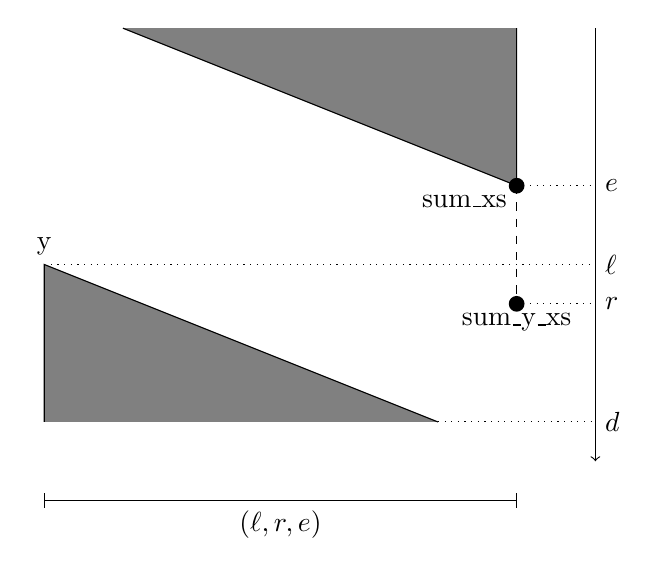
\begin{tikzpicture}
    \def\T{5}
    \def\E{3}
    \def\Ld{2}
    \def\Rd{1.5}
    \def\B{0}
    \def\BB{-1}

    \def\L{0}
    \def\R{6}
    \def\A{7}

    \def\Top{(\L+1,\T) -- (\R,\E) -- (\R,\T)}
    \fill[gray] \Top -- cycle;
    \draw\Top;

    \def\Bot{(\L,\B) -- (\L,\Ld) -- (\R-1,\B)}
    \fill[gray] \Bot -- cycle;
    \draw\Bot;

    \draw[dashed] (\R,\E) -- (\R,\Rd);

    \foreach \x/\y/\z in {
      (\R,\E)/below left/\lst$sum_xs$,
      (\R,\Rd)/below/\lst$sum_y_xs$}
      \fill \x circle (.1) node[\y] {\z};

    \node[above] at (\L,\Ld) {\lst$y$};
    
    \draw[->] (\A,\T) -- (\A,\B-.5);

    \draw[dotted] (\R,\E) -- (\A,\E) node[right] {$e$};
    \draw[dotted] (\L,\Ld) -- (\A,\Ld) node[right] {$\ell$};
    \draw[dotted] (\R,\Rd) -- (\A,\Rd) node[right] {$r$};
    \draw[dotted] (\R-1,\B) -- (\A,\B) node[right] {$d$};

    \draw[|-|] (\L,\BB) to node[below] {$(\ell,r,e)$} (\R,\BB);
  \end{tikzpicture}
  \caption{\lst$slice' d l r e$}
\end{figure}

\begin{figure}
  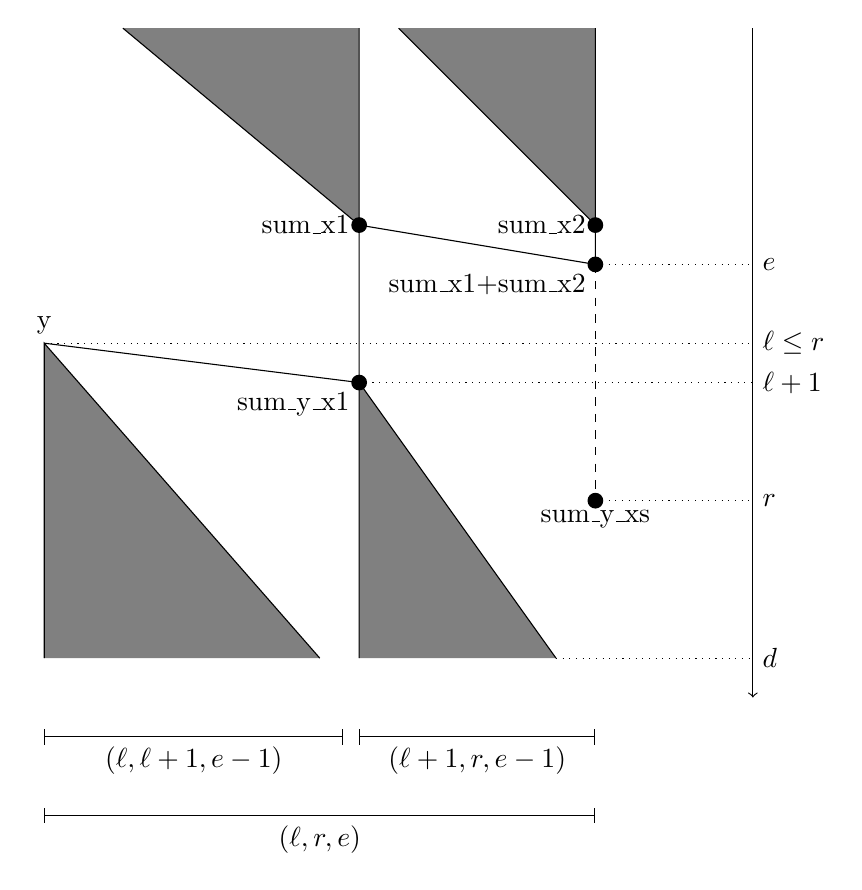
\begin{tikzpicture}
    \def\T{8}
    \def\E{5}
    \def\Ld{4}
    \def\Rd{2}
    \def\B{0}
    \def\BB{-1}

    \def\L{0}
    \def\M{4}
    \def\R{7}
    \def\A{9}

    \def\LTop{(\L+1,\T) -- (\M,\E+.5) -- (\M,\T)}
    \fill[gray] \LTop -- cycle;
    \draw\LTop;

    \def\RTop{(\M+.5,\T) -- (\R,\E+.5) -- (\R,\T)}
    \fill[gray] \RTop -- cycle;
    \draw\RTop;

    \def\LBot{(\L,\B) -- (\L,\Ld) -- (\M-.5,\B)}
    \fill[gray] \LBot -- cycle;
    \draw\LBot;

    \def\RBot{(\M,\B) -- (\M,\Ld-.5) -- (\R-.5,\B)}
    \fill[gray] \RBot -- cycle;
    \draw\RBot;

    \draw (\M,\E+.5) -- (\R,\E) -- (\R,\E+.5);
    \draw (\L,\Ld) -- (\M,\Ld-.5) -- (\M,\E+.5);

    \draw[dashed] (\R,\E) -- (\R,\Rd);

    \foreach \x/\y/\z in {
      (\M,\E+.5)/left/\lst$sum_x1$,
      (\R,\E+.5)/left/\lst$sum_x2$,
      (\R,\E)/below left/\lst$sum_x1+sum_x2$,
      (\M,\Ld-.5)/below left/\lst$sum_y_x1$,
      (\R,\Rd)/below/\lst$sum_y_xs$}
      \fill \x circle (.1) node[\y] {\z};

    \node[above] at (\L,\Ld) {\lst$y$};
    
    \draw[->] (\A,\T) -- (\A,\B-.5);

    \draw[dotted] (\R,\E) -- (\A,\E) node[right] {$e$};
    \draw[dotted] (\L,\Ld) -- (\A,\Ld) node[right] {$\ell\leq r$};
    \draw[dotted] (\M,\Ld-.5) -- (\A,\Ld-.5) node[right] {$\ell+1$};
    \draw[dotted] (\R,\Rd) -- (\A,\Rd) node[right] {$r$};
    \draw[dotted] (\R-.5,\B) -- (\A,\B) node[right] {$d$};

    \draw[|-|] (\L,\BB) to node[below] {$(\ell,\ell+1,e-1)$} (\M-.2,\BB);
    \draw[|-|] (\M,\BB) to node[below] {$(\ell+1,r,e-1)$} (\R,\BB);
    \draw[|-|] (\L,\BB-1) to node[below] {$(\ell,r,e)$} (\R,\BB-1);
  \end{tikzpicture}
  \caption{\lst$slice' d l r e | l <= r == sliceLeft d l r e$\\
  \lst$sum_y_x1 = y + sum_x1$}
\end{figure}

\begin{figure}
  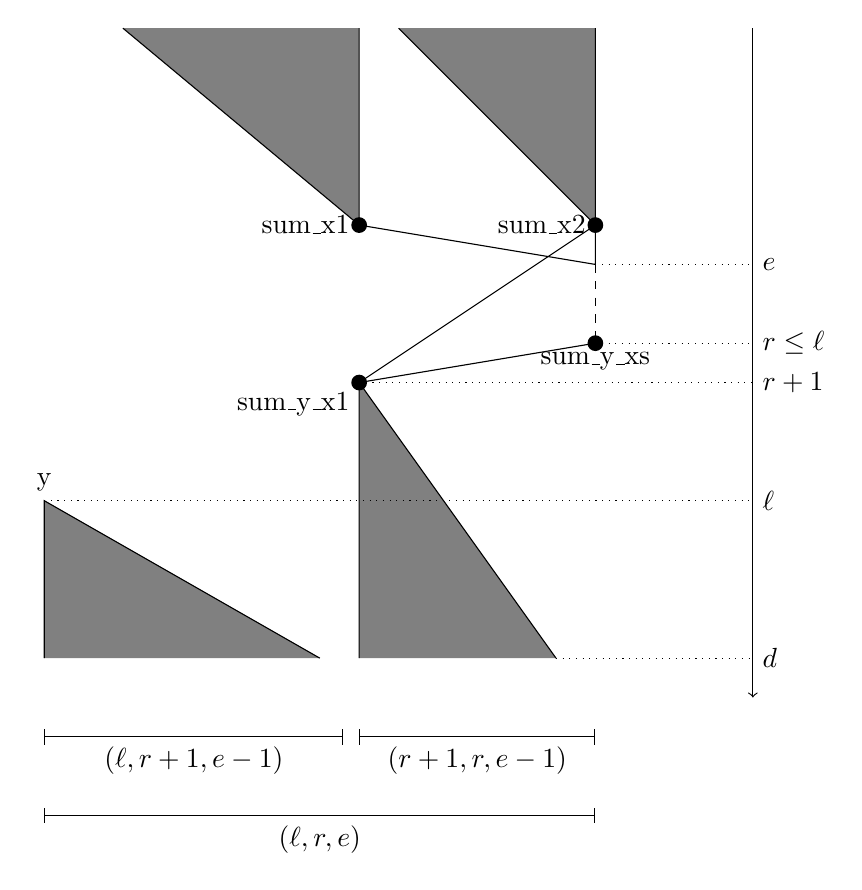
\begin{tikzpicture}
    \def\T{8}
    \def\E{5}
    \def\Ld{2}
    \def\Rd{4}
    \def\B{0}
    \def\BB{-1}

    \def\L{0}
    \def\M{4}
    \def\R{7}
    \def\A{9}

    \def\LTop{(\L+1,\T) -- (\M,\E+.5) -- (\M,\T)}
    \fill[gray] \LTop -- cycle;
    \draw\LTop;

    \def\RTop{(\M+.5,\T) -- (\R,\E+.5) -- (\R,\T)}
    \fill[gray] \RTop -- cycle;
    \draw\RTop;

    \def\LBot{(\L,\B) -- (\L,\Ld) -- (\M-.5,\B)}
    \fill[gray] \LBot -- cycle;
    \draw\LBot;

    \def\RBot{(\M,\B) -- (\M,\Rd-.5) -- (\R-.5,\B)}
    \fill[gray] \RBot -- cycle;
    \draw\RBot;

    \draw (\M,\E+.5) -- (\R,\E) -- (\R,\E+.5);
    \draw (\R,\E+.5) -- (\M,\Rd-.5) -- (\R,\Rd);

    \draw[dashed] (\R,\E) -- (\R,\Rd);

    \foreach \x/\y/\z in {
      (\M,\E+.5)/left/\lst$sum_x1$,
      (\R,\E+.5)/left/\lst$sum_x2$,
      %(\R,\E)/below left/\lst$sum_x1+sum_x2$,
      (\M,\Rd-.5)/below left/\lst$sum_y_x1$,
      (\R,\Rd)/below/\lst$sum_y_xs$}
      \fill \x circle (.1) node[\y] {\z};

    \node[above] at (\L,\Ld) {\lst$y$};
    
    \draw[->] (\A,\T) -- (\A,\B-.5);

    \draw[dotted] (\R,\E) -- (\A,\E) node[right] {$e$};
    \draw[dotted] (\L,\Ld) -- (\A,\Ld) node[right] {$\ell$};
    \draw[dotted] (\M,\Rd-.5) -- (\A,\Rd-.5) node[right] {$r+1$};
    \draw[dotted] (\R,\Rd) -- (\A,\Rd) node[right] {$r\leq \ell$};
    \draw[dotted] (\R-.5,\B) -- (\A,\B) node[right] {$d$};

    \draw[|-|] (\L,\BB) to node[below] {$(\ell,r+1,e-1)$} (\M-.2,\BB);
    \draw[|-|] (\M,\BB) to node[below] {$(r+1,r,e-1)$} (\R,\BB);
    \draw[|-|] (\L,\BB-1) to node[below] {$(\ell,r,e)$} (\R,\BB-1);
  \end{tikzpicture}
  \caption{\lst$slice' d l r e | l > r == sliceRight d l r e$\\
  \lst$sum_y_x1 = sum_y_xs - sum_x2$}
\end{figure}

\begin{table}
  \begin{tabular}{| r || r | r | r |}
    \hline
    Depth &      C & Ladner-Fischer & Minimum \\
    \hline
        3 &     12 &             12 &      12 \\
        4 &     31 &             31 &      31 \\
        5 &     74 &             74 &      74 \\
        6 &    168 &            168 &     167 \\
        7 &    369 &            369 &     364 \\
        8 &    793 &            792 &     773 \\
        9 &   1679 &           1672 &    1614 \\
       10 &   3518 &           3487 &    3327 \\
       11 &   7315 &           7206 &    6800 \\
       12 &  15122 &          14788 &   13809 \\
       13 &  31120 &          30185 &   27922 \\
       14 &  63814 &          61356 &   56275 \\
       15 & 130481 &         124308 &  113172 \\
       16 & 266176 &         251199 &  227221 \\
       17 & 541953 &         506578 &  455702 \\
       18 &      - &        1019920 &  913175 \\
       19 &      - &        2050785 & 1828888 \\
       20 &      - &        4119280 & 3661337 \\
    \hline              
  \end{tabular}         
  \caption{More values could be computed in the first column using memoization
  and other optimizations.}
\end{table}


\end{document}
